\newpage
\subsection{}

    Rough steps:
    \begin{enumerate}
        \item Read string from console
        \item Tokenize string (Read chars until operator is found, substrings between operators are constants or variables)
        \item Parse token-stream to operator tree (e.g. with Dijkstra's famous shunting yard algorithm)
        \item Optionally post process operator tree to simplify it
    \end{enumerate}

    \begin{figure}[H]
        \centering
        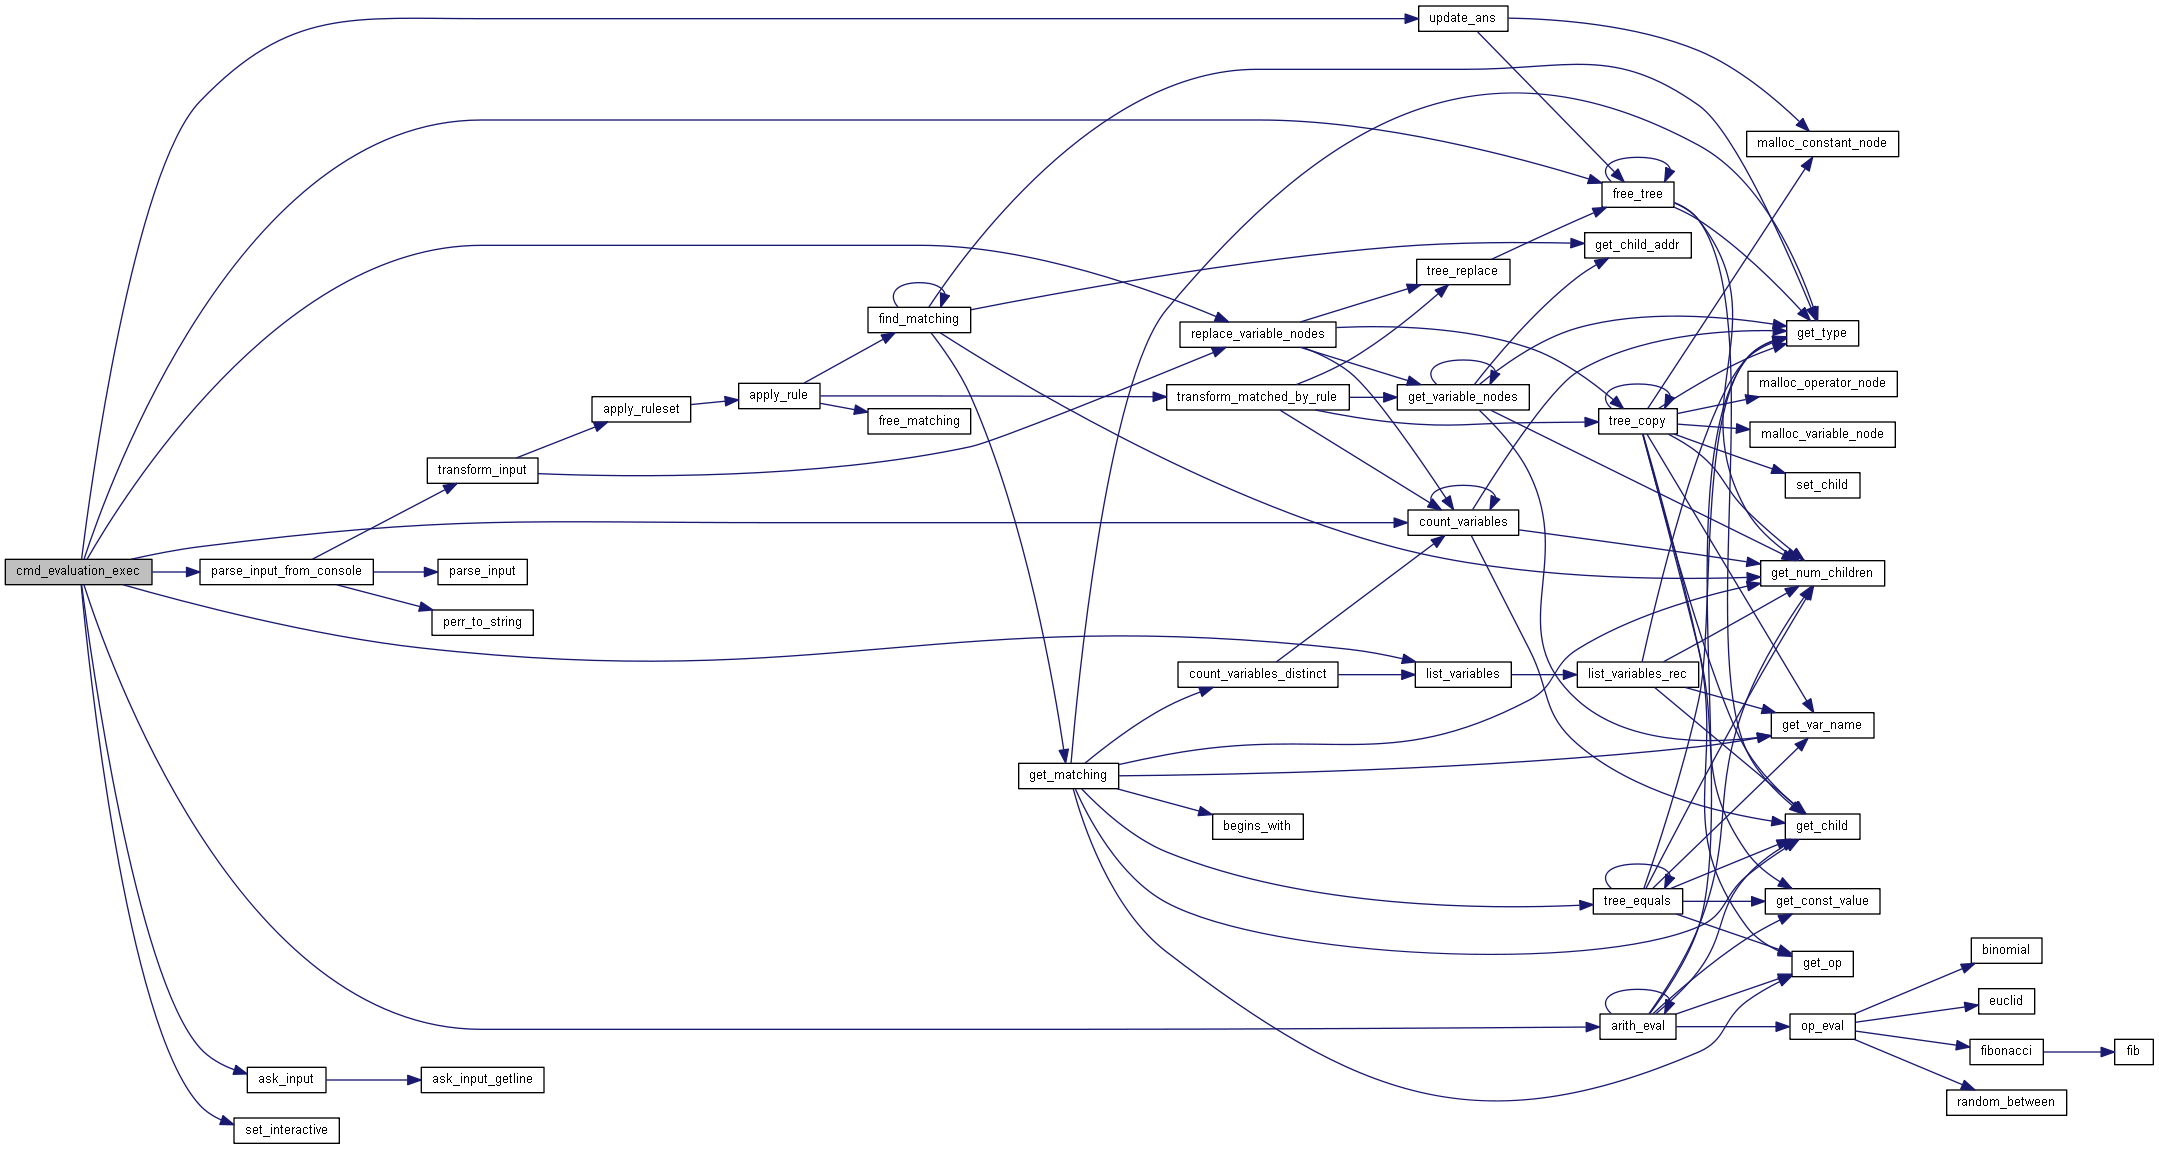
\includegraphics[width=\linewidth]{images/ex7/read_and_simplify.png}
        \caption{To read string from console and simplify it (step 1 and 4)}
    \end{figure}

    \begin{figure}[H]
        \centering
        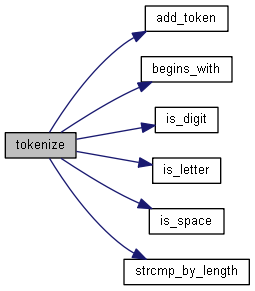
\includegraphics[width=0.3\linewidth]{images/ex7/tokenize.png}
        \caption{To tokenize it (step 2)}
    \end{figure}

    \begin{figure}[H]
        \centering
        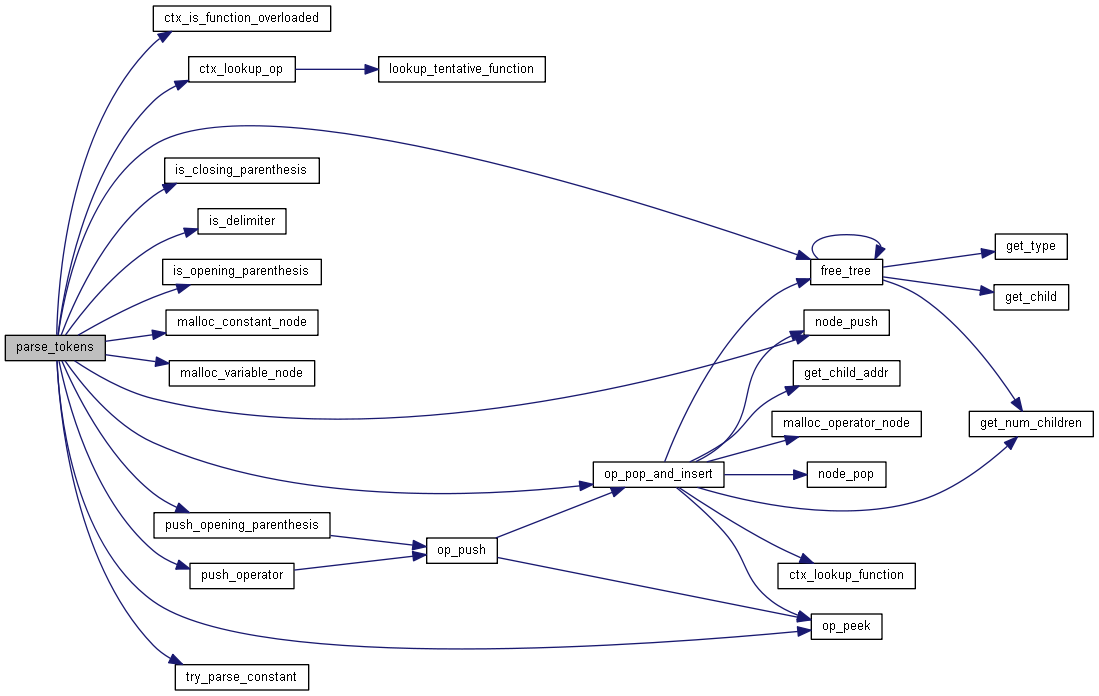
\includegraphics[width=\linewidth]{images/ex7/parse.png}
        \caption{To parse it (step 3)}
    \end{figure}

\subsection{2}
See given Java code

\subsection{3}
See given Java code